\section*{Generative Models}

- Given data sample $x$ 

- Discriminative model predict $y arrow$ conditional distribution $p(y \mid x)$. 

- Generative models $arrow$ distribution $p(x)$ defined over the datapoints $x$. Generative models  categories: explicit (explicitly model the probability distribution) or implicit (generate samples according to $p$).

- Taxonomy: 

\includegraphics*[width=0.9\columnwidth]{figures/generative_taxonomy.png}


\begin{itemize}
  \item Implicit density models (GANs), high-quality, realistic samples, challenging to train (mode collapse model fails to capture the diversity of the data distribution)

  \item Tractable density models, (Autoregressive models and Normalizing Flows), exact likelihood computation, (beneficial for tasks that require likelihood evaluation and interpretability). Autoregressive models generate data sequentially, slow in sampling. Normalizing Flows, more efficient sampling and inference (using invertible transformations), computationally intensive to train.

  \item Approximate models, (VAEs and Energy-based models). VAEs optimize a lower bound on the likelihood $arrow$ easier and more stable training than GANs but less sharp samples.

  \item Diffusion models $arrow$ hybrid approach, iteratively convert noise into samples via a reverse Markov process, highquality images and audio, slow at sampling time.

\end{itemize}

- trade-off between sample quality, sampling speed, and diversity.

\includegraphics*[width=0.4\columnwidth]{figures/generative_pros_cons.png}


\subsubsection*{Generative Adversarial Networks}
\includegraphics*[width=0.9\columnwidth]{figures/generative_GAN.png}

- two models: a generator $G$ with paramters $\boldsymbol{\theta}$ and a discriminator $D$ with parameters $\boldsymbol{\varphi}$. 

- G learns to generate samples from the data distribution $p_{d}$, while D learns to distinguish between real and fake samples. 

- Therefore, contrary to singleobjective minimization $f: \mathcal{X} arrow \mathbb{R}$, the optimization of a GAN is formulated as a differentiable two-player game where the generator $G$, and the discriminator $D$, aim at minimizing their own cost function $\mathcal{L}^{\boldsymbol{\theta}}$ and $\mathcal{L}^{\varphi}$, respectively, as follows:

$\boldsymbol{\theta}^{\star} \in \underset{\boldsymbol{\theta} \in \Theta}{\arg \min } \mathcal{L}^{\boldsymbol{\theta}}(\boldsymbol{\theta}, \boldsymbol{\varphi}^{\star}) \quad \boldsymbol{\varphi}^{\star} \in \underset{\boldsymbol{\varphi} \in \Phi}{\arg \min } \mathcal{L}^{\boldsymbol{\varphi}}(\boldsymbol{\theta}^{\star}, \boldsymbol{\varphi})$


- When $\mathcal{L}^{\boldsymbol{\theta}}=-\mathcal{L}^{\varphi}$ the game is called a zero-sum game and (2Player-Game) is a minmax problem.

\begin{enumerate}
  \item The discriminator "distinguishes" real vs. fake samples:
\end{enumerate}

$p_{z}$ known "noise" distribution, e.g. $\mathcal{N}(0,1)$

$p_{d}$ the real data distribution

$D: x \mapsto y \in[0,1]$, where $y$ is an estimated probability that $x \sim p_{d}$

\begin{enumerate}
  \setcounter{enumi}{1}
  \item The generator aims at fooling the discriminator that its samples are real:
\end{enumerate}

$G: z \mapsto x$, such that if $z \sim p_{z}$, then hopefully $x \sim p_{d}$

$p_{g}$ the "fake" data distribution

\begin{enumerate}
  \setcounter{enumi}{2}
  \item Objective
  $
  \min _{G} \max _{D} \underset{x \sim p_{d}}{\mathbb{E}}[\log D(x)]+\underset{z \sim p_{z}}{\mathbb{E}}[\log (1-D(G(z)))]
  $
\end{enumerate}



\begin{itemize}
  \item Loss for $D$ : distinguish between $x \sim p_{g}$ and $x \sim p_{d}$ (binary classification):
\end{itemize}

$\mathscr{L}_{D}(G, D)=\max _{D} \underset{x \sim p_{d}}{\mathbb{E}}[\log D(x)]+\underset{z \sim p_{z}}{\mathbb{E}}[\log (1-D(G(z)))]$

\begin{itemize}
  \item Loss for $G$ : fool $D$ that $G(z) \sim p_{d}$ :
\end{itemize}

$
\begin{aligned}
\mathscr{L}_{G}(G, D) & =\min _{G} \underset{z \sim p_{z}}{\mathbb{E}}[\log (1-D(G(z)))] \\
& :=(\text { in practice }) \max _{G} \underset{z \sim p_{z}}{\mathbb{E}}[\log (D(G(z)))]
\end{aligned}
$

\begin{enumerate}
  \setcounter{enumi}{3}
  \item Theoretical Solution: The optimum is reached when $p_{g}=p_{d}$ and the optimal value is $-\log 4$
\end{enumerate}

\subsubsection*{Alternating-GAN algorithm}

\begin{wrapfigure}{r}{0.5\columnwidth} 
    \centering
    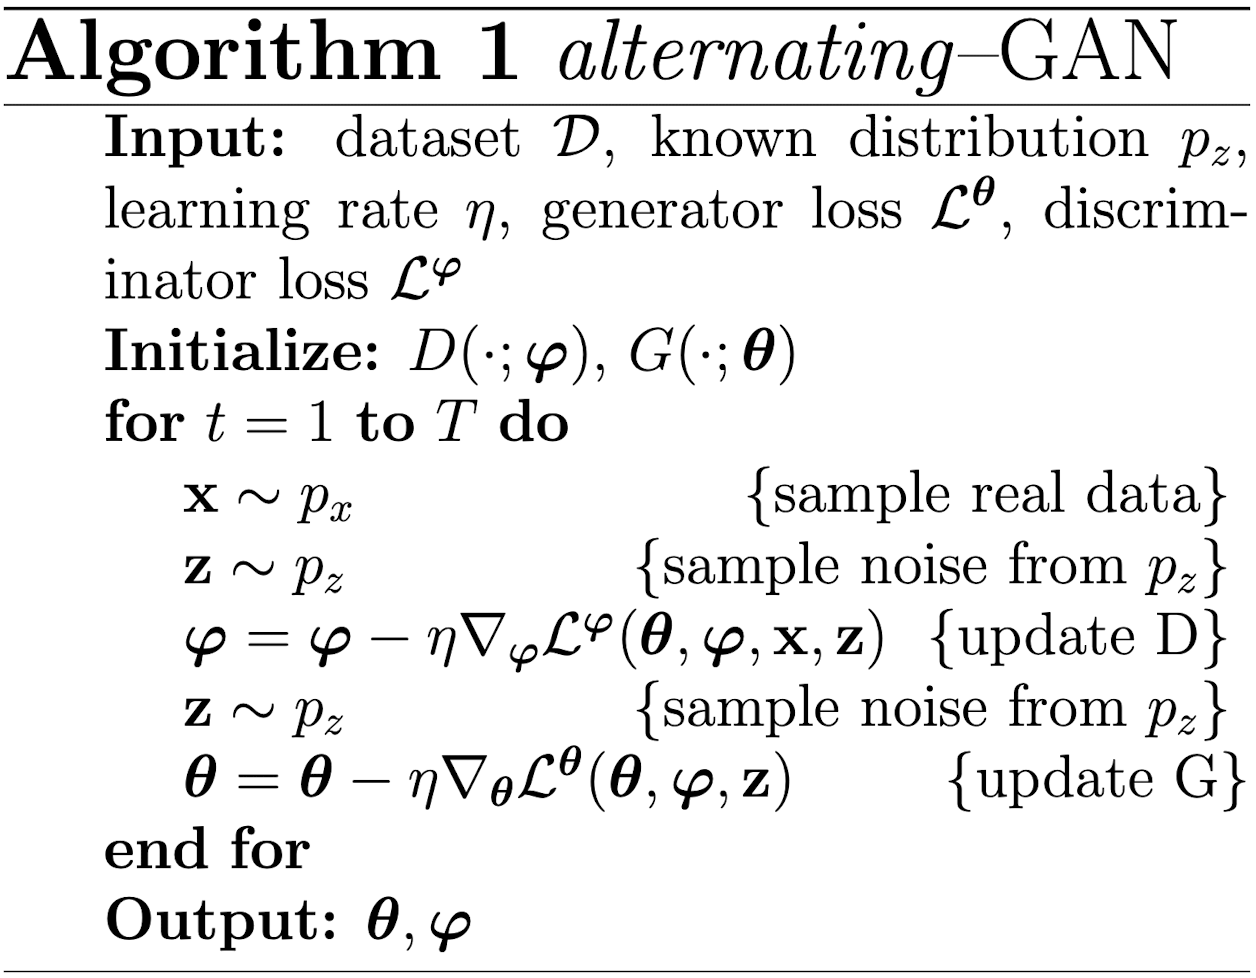
\includegraphics[width=0.5\columnwidth]{figures/generative_alter_GAN.png}
    \vspace{-10pt}
\end{wrapfigure}

- $G$ : deep neural network $G(\mathbf{z} ; \boldsymbol{\theta})$ with parameters $\boldsymbol{\theta}$

- $D$ : deep neural network $D(\mathbf{x} ; \boldsymbol{\varphi})$ with parameters $\varphi$

- In most GAN implementations $G$ and $D$ have different losses $\mathcal{L}^{\theta}$ and $\mathcal{L}^{\varphi a}$, resp.

% \includegraphics*[width=\columnwidth]{figures/generative_alter_GAN.png}

% For simplicity, in Alg. 1 we used gradient descent, however in practice GANs are often optimized using Adam [Kingma and Ba, 2015], and developing well performing minimax optimization methods is an active research area.
% \footnotetext{${ }^{a}$ Although we minimize both the loses, this notation generalizes the zero-sum game, as the latter holds when $\mathcal{L}^{\theta}=-\mathcal{L}^{\varphi}:=\mathcal{L}$.
% }

\subsubsection*{Conditional GAN - (CGAN)}
\includegraphics*[width=0.9\columnwidth]{figures/generative_CGAN.png}

- Applications requiring conditional probability distribution (e.g. "in-painting", segmentation, predicting the next frame of a video etc.).

- In CGANs both the Generator and the Discriminator are conditioned during training by some additional information, typically the class labels (but could also be images e.g. auto-generated edges of an image, conditioning on non-occluded portion-so as to generate the occluded part of the image etc).

- When conditioning on the class labels, typically one-hot vector representation of the class labels is used (empirically shown to perform better).

\subsubsection*{GAN architectures for images}

\includegraphics*[width=1\columnwidth]{figures/generative_GAN_architecture.png}

- Deep Convolutional GANs - DCGAN. Notably, 

- G uses transposed convolutional layer (a.k.a. fractionally strided convolutions), also informally called "Deconvolution layers" (wrongfully). 

- Simplest way to explain these is that they "swap" the forward and the backward passes of a convolution layer: the forward transposed convolution operation can be thought of as the gradient of some convolution with respect to its input, which is usually how transposed convolutions are also implemented in practice.


\subsubsection*{Diffusion models}

\includegraphics*[width=1\columnwidth]{figures/generative_diffusion.jpg}

- implementation in AI image generators like DALL-E 3, Stable Diffusion, and Midjourney. 

- Unlike GANs, work by progressively adding noise to input data and training one single model to estimate the added noise and recover the data.


- Consider a Markov chain with $X_{0} \sim p_{0}$ and a forward transition s.t. $X_{t+1} \sim p(\cdot \mid X_{t})$ then we call \textbf{forward decomposition}:

$
p(x_{0: T})=p_{0}(x_{0}) \prod_{t=0}^{T-1} p(x_{t+1} \mid x_{t})
$

where at each step, the marginal distribution of $X_{t}$ satisfies:
$
p(x_{t})=\int p(x_{t} \mid x_{t-1}) p(x_{t-1}) \mathrm{d} x_{t-1}
$

- backward transition can be obtained with Bayes' rule 

$p(x_{t} \mid x_{t+1})=$ $p(x_{t+1} \mid x_{t}) p(x_{t}) / p(x_{t+1})$, 

and we call \textbf{backward decomposition}:

$
p(x_{0: T})=p_{T}(x_{T}) \prod_{t=0}^{T-1} p(x_{t} \mid x_{t+1})
$

- A generative model can be constructed sampling from $p(x_{0: T})$ using \textbf{ancestral sampling}:

Sample $X_{T} \sim p_{T}(\cdot)$ then:
for $k=T-1, \ldots, 0$ :
Sample $\quad X_{t} \sim p(\cdot \mid X_{t+1})$

\begin{itemize}
  \item We consider $p_{0}=p_{\text {data }} \in \mathcal{P}(\mathbb{R}^{d})$

  \item We chose the forward transition to be Gaussian $p(x_{t+1} \mid x_{t})=\mathcal{N}(x_{t+1} ; \alpha x_{t},(1-.$ $..\alpha^{2}) \mathbb{I}_{d})$

  \item The conditional $p(x_{t} \mid x_{0})$ is also Gaussian $\mathcal{N}(x_{t} ; \alpha^{t} x_{0},(1-\alpha^{2 t}) \mathbb{I}_{d})$

  \item The Markov chain converges to $p_{\text {ref }}=$ $\mathcal{N}(x ; 0, \mathbb{I}_{d})$ for $T arrow \infty$.

  \item Therefore for $\mathrm{T}$ large enough $p_{T}(x) \approx$ $p_{\text {ref }}(x)$

  \item To generate samples we use ancestral sampling replacing $p_{T}$ with $p_{\text {ref}}$

\end{itemize}

- Key problem: the backward transition $p(x_{t} \mid x_{t+1})$ can't be computed, we need an approximation!

- Using a Taylor expansion we can approximate the backward transition:
$p(x_{t} \mid x_{t+1})=p(x_{t+1} \mid x_{t}) \exp [\log p(x_{t})-\log p(x_{t+1})] \approx \mathcal{N}(x_{t} ;(2-\alpha) x_{t+1}+(1-\alpha^{2}) \underbrace{\nabla \log p(x_{t+1})}_{\text{Score}},(1-\alpha^{2}) \mathbb{I}_{d})$


\subsubsection*{Denoising score matching}
- The Stein Score is analytically intractable, but we can approximate it using a NN $s_{\theta}(x_{t})$. 

- Surprisingly, we can learn the score solving a simple regression problem via the Denoising Score Matching (DSM) loss:
$\theta^{\star}=\underset{\theta}{\arg \min } \mathcal{L}(\theta):=\frac{1}{2} \mathbb{E}_{X_{t}}[\|\nabla \log p(X_{t})-s_{\theta}(X_{t})\|^2]$


- Problem still intractable: we do not have access to the marginal $p(x_{t})$ at each step but we can manipulate it:

\scalebox{0.7}{
$
\begin{aligned}
\mathcal{L}(\theta) & =\mathrm{C}_{1}+\frac{1}{2} \mathbb{E}_{X_{t}}[\|s_{\theta}(X_{t})\|^{2}]-\mathbb{E}_{X_{t}}[\nabla \log p(X_{t})^{\top} s_{\theta}(X_{t})] \\
& =\mathrm{C}_{1}+\frac{1}{2} \mathbb{E}_{X_{t}}[\|s_{\theta}(X_{t})\|^{2}]-\int \nabla \log p(X_{t})^{\top} s_{\theta}(X_{t}) p(X_{t}) \mathrm{d} x_{t}
\end{aligned}
$
}

% $\mathcal{L}(\theta) = \mathrm{C}_{1} + \frac{1}{2} \mathbb{E}_{X_{t}}[\|s_{\theta}(X_{t})\|^2] - \mathbb{E}_{X_{t}}[\nabla \log p(X_{t})^{\top} s_{\theta}(X_{t})] = \mathrm{C}_{1} + \frac{1}{2} \mathbb{E}_{X_{t}}[\|s_{\theta}(X_{t})\|^2] - \int \nabla \log p(X_{t})^{\top} s_{\theta}(X_{t}) p(X_{t}) \mathrm{d} x_{t}$


- Using that $p(x_{t})=\int p_{0}(x_{0}) p(x_{t} \mid x_{0}) \mathrm{d} x_{0}$ we get:

$
\nabla \log p(X_{t})=\mathbb{E}_{X_{0} \mid X_{t}}[\nabla \log p(X_{t} \mid X_{0})]
$

Substituding in the DSM-loss:

\scalebox{0.7}{
$
\begin{aligned}
\mathcal{L}(\theta) & =\mathrm{C}_{1}+\frac{1}{2} \mathbb{E}_{X_{t}}[\|s_{\theta}(X_{t})\|^{2}]-\mathbb{E}_{X_{0}} \mathbb{E}_{X_{t} \mid X_{0}}[\nabla \log p(X_{t} \mid X_{0})^{\top} s_{\theta}(X_{t})] \\
& =\mathrm{C}_{1}+\frac{1}{2} \mathbb{E}_{X_{0}} \mathbb{E}_{X_{t} \mid X_{0}}[\|s_{\theta}(X_{t})-\nabla \log p(X_{t} \mid X_{0})\|^{2}] \\
& -\frac{1}{2} \underbrace{\mathbb{E}_{X_{0}} \mathbb{E}_{X_{t} \mid X_{0}}[\|\nabla \log p(X_{t} \mid X_{0})\|^{2}]}_{\text {const. }} \\
& =\mathrm{C}_{2}+\frac{1}{2} \mathbb{E}_{X_{0}} \mathbb{E}_{X_{t} \mid X_{0}}[\|s_{\theta}(X_{t})-\nabla \log p(X_{t} \mid X_{0})\|^{2}]
\end{aligned}
$
}

- In practice we estimate all the scores simultaneously i.e. $s_{\theta^{\star}}(t, X_{t})$ such that:

$\theta^* = \underset{\theta}{\arg\min} \frac{1}{2} \sum_{t=1}^{T} \mathbb{E}_{X_0} \mathbb{E}_{X_t \mid X_0}[\|s_\theta(t, X_t) - \nabla \log p(X_t \mid X_0)\|^2]$

- Recalling now our choice of forward transition for which $p(x_{t} \mid x_{0})=\mathcal{N}(x_{t} ; \alpha^{t} x_{0},(1-. ..\alpha^{2 t}) \mathbb{I}_{d})$ :

\begin{itemize}
  \item $\nabla \log p(x_{t} \mid x_{0})=-\frac{(x_{t}-\alpha^{t} x_{0})}{(1-\alpha^{2 t})}$

  \item $X_{t}=\alpha^{t} X_{0}+\sqrt{1-\alpha^{2 t}} \xi_{t} \xi_{t} \sim \mathcal{N}(0, \mathbb{I}_{d})$

  \item $\nabla \log p(X_{t} \mid X_{0})=-\frac{\xi_{t}}{\sqrt{1-\alpha^{2 t}}}$

\end{itemize}

- parameterize the score function as $s_{\theta}(t, X_{t})=-\frac{\hat{\xi}_{\theta}(t, X_{t})}{\sqrt{1-\alpha^{2 t}}}$ then the problem is equivalent to:

$
\theta^{\star}=\underset{\theta}{\arg \min } \frac{1}{2} \sum_{k=1}^{T} \mathbb{E}_{X_{0}} \mathbb{E}_{X_{t} \mid X_{0}}[\|\hat{\xi}_{\theta}(t, X_{t})-\xi_{t}\|^{2}]
$

which has the illuminating interpretation of learning to predict the added noise $\xi_{t}$ from the noised data $X_{t}$.

- Finally, we can generate new samples from the backward process by sampling $X_{T} \sim p_{\text {ref }}$ and using the approximation of the backward transition and the learned score to perform ancestral sampling:

$
X_{t}=(2-\alpha) X_{t+1}+(1-\alpha^{2}) s_{\theta^{\star}}(t+1, X_{t+1})+\sqrt{1-\alpha^{2}} \xi_{t+1} \quad \xi_{t+1} \sim \mathcal{N}(0, \mathbb{I}_{d})
$

\subsubsection*{Implementation}

\includegraphics*[width=\columnwidth]{figures/generative_diffusion_architecture.jpg}

- Diffusion models often use a U-net architecture with ResNet blocks and self attention layers to represent the score function $\hat{\xi}_{\theta}(t, X_{t})$.

- The time step can be represented with sinusoidal positional encodings as done for transformers or with random Fourirer features. 

- The time features are then fed to the residual blocks using either spatial addition or adaptive group normalization layers.

\subsubsection*{Training and Sampling}

\includegraphics*[width=\columnwidth]{figures/generative_diffusion_training_sampling.png}

% \subsubsection*{Algorithm 2 Training}
% Input: Data distribution $p_{0}, \alpha$

% Output: Learned parameters $\theta^{*}$

% Initialize: Parameters $\theta$

% repeat

% Sample initial data $X_{0} \sim p_{0}$

% Sample time step $t \sim \operatorname{Uniform}(\{1, \ldots, T\})$

% Sample noise $\xi_{t} \sim \mathcal{N}(0, \mathbb{I}_{d})$

% Update $\theta$ using gradient descent step on:

% $\nabla_{\theta} \frac{1}{2} \mathbb{E}_{X_{0}} \mathbb{E}_{X_{t} \mid X_{0}}[\|s_{\theta}(t, \alpha^{t} X_{0}+\sqrt{1-\alpha^{2 t}} \xi_{t})-\xi_{t}\|^{2}]$ until convergence

% \subsubsection*{Algorithm 3 Sampling}
% Input: Learned parameters $\theta^{*}, p_{\text {ref }}, \alpha$

% Output: Generated sample $X_{0}$

% Sample $X_{T} \sim p_{\text {ref }}$

% for $t=T-1$ to 0 do

% Sample noise $\xi_{t+1} \sim \mathcal{N}(0, \mathbb{I}_{d})$ :

% $
% \begin{aligned}
% & X_{t}=(2-\alpha) X_{t+1}+(1-\alpha^{2}) s_{\theta^{\star}}(t+1, X_{t+1})+ \\
% & \sqrt{1-\alpha^{2}} \xi_{t+1}
% \end{aligned}
% $

% end for

\subsubsection*{Exponential moving average}
- The training of the U-net via Denoising Score Matching can be very unstable. 

- To regularize it, usually an exponential moving average of the weights is used along the training:

$
\bar{\theta}_{n+1}=(1-\beta) \bar{\theta}_{n}+\beta \theta_{n}
$

where $\beta$ regulates the rate of forgetting of the initial conditions.

\subsubsection*{Conditional training}

- for diffusion models, conditioning is done by adding an additional input to the score function such that a conditional score is learned:

$\theta^{\star}=\underset{\theta}{\arg \min } \frac{1}{2} \sum_{k=1}^{T} \mathbb{E}_{X_{0}, Y} \mathbb{E}_{X_{t} \mid X_{0}}[\|s_{\theta}(t, X_{t}^{Y} ; Y)-\nabla \log p(X_{t}^{Y} \mid X_{0}^{Y})\|^{2}]$

- conditioning is fed into the network in a similar way than the time features

\subsubsection*{Applications of GANs and Diffusion Models}
Image generation and editing, art creation, data augmentation, adversarial examples, drug discovery, protein structure prediction, anomaly detection, weather forecasting, video generation, voice synthesis and modification, restoration of old photographs and artworks, fashion design, architectural visualization, gaming, virtual reality and augmented reality, language translation and interpretation, financial modeling.

% GANs and diffusion models have also been used for other data modalities: For raw-waveform audio synthesis, examples include WaveGAN [Donahue et al., 2019] and MelGAN [Kumar et al., 2019], among others. For generating realistic tabular data, see e.g. [Kotelnikov et al., 2022].

% \subsubsection*{Summary}
% We have studied:

% \begin{enumerate}
%   \item Generative models

%   \item Generative Adversarial Networks

% \end{enumerate}

% \begin{itemize}
%   \item Players (generator \& discriminator)
%   \item Objectives
%   \item Solution \& Algorithm, Conditional GANs
% \end{itemize}

% \begin{enumerate}
%   \setcounter{enumi}{2}
%   \item Diffusion models
% \end{enumerate}

% \begin{itemize}
%   \item Ancestral sampling
%   \item Denoising Score Matching
%   \item Conditional training
% \end{itemize}

% \subsubsection*{Additional Notes (optional material) 
%  $\mathrm{KL}$ and JS divergences}
% Before proving that at the equilibrium of the above GAN framework $p_{g}=p_{d}$ we need to define some measures of similarity between two probability distributions: The KL and JS divergences.

% The Kullback-Leibler (KL) divergence is defined as:

% $
% \mathbb{D}_{K L}(p_{d} \| p_{g}):=\int_{x} \log (\frac{p_{d}(x)}{p_{g}(x)}) p_{d}(x) \mathrm{d} x .
% $

% KL is also called relative entropy, as it measures how one probability distribution is different from a "reference" probability distribution, and it is asymmetric.

% The Jenson-Shannon (JS) divergence is defined as:

% $\mathbb{D}_{J S}(p \| q):=\frac{1}{2} \mathbb{D}_{K L}(p \| \frac{p+q}{2})+\frac{1}{2} \mathbb{D}_{K L}(q \| \frac{p+q}{2})$

% Note that contrary to the KL divergence defined above, the JS divergence is symmetric.

% \subsubsection*{The GAN framework: 
%  Equilibrium at $p_{g}=p_{d}$}
% In the following, we'll assume the neural network models $\mathrm{G}$ and $\mathrm{D}$ have infinite capacity, so can represent any probability distribution. We will study the convergence of the loss function in the space of probability density functions.

% The discriminator maximizes:

% $
% \begin{aligned}
% \mathcal{L}(G, D) & =\int_{x} p_{d}(x) \log (D(x)) \mathrm{d} x+\int_{z} p_{z}(z) \log (1-D(G(z))) \mathrm{d} z \\
% & =\int_{x} p_{d}(x) \log (D(x))+p_{g}(x) \log (1-D(x)) \mathrm{d} x
% \end{aligned}
% $

% Where we used $x=G(z)$, and $p_{g}$ is the distribution of $x$.

% The above integrand can be written as: $f(y)=a \log y+b \log (1-y)$. To solve for its critical points: $f^{\prime}(y)=0 arrow \frac{a}{y}-\frac{b}{1-y}=$ $0 arrow y=\frac{a}{a+b}$. Moreover, if $a+b \neq 0$ we obtain that $\frac{a}{a+b}$ is a maximum as $f^{\prime \prime}(\frac{a}{a+b})<0$. Hence, optimal discriminator $D^{\star}$ is:

% $
% D^{\star}(x)=\frac{p_{d}(x)}{p_{d}(x)+p_{g}(x)}
% $

% By replacing the optimal discriminator in the above objective, we obtain that the generator minimizes:

% $
% \begin{aligned}
% \mathcal{L}(G, D^{\star}) & =\underset{x \sim p_{d}}{\mathbb{E}}[\log D^{\star}(x)]+\underset{x \sim p_{g}}{\mathbb{E}}[\log (1-D^{\star}(x))] \\
% & =\underset{x \sim p_{d}}{\mathbb{E}}[\log \frac{p_{d}(x)}{p_{d}(x)+p_{g}(x)}]+\underset{x \sim p_{g}}{\mathbb{E}}[\log \frac{p_{g}(x)}{p_{d}(x)+p_{g}(x)}] \\
% & =-\log 4+\mathbb{D}_{K L}(p_{d} \| \frac{p_{d}+p_{g}}{2})+\mathbb{D}_{K L}(p_{g} \| \frac{p_{d}+p_{g}}{2}) \\
% & =-\log 4+2 \cdot \mathbb{D}_{J S}(p_{d} \| p_{g})
% \end{aligned}
% $

% where to obtain the third expression we used the definition of logarithm:

% $
% \begin{aligned}
% & \log 2+\log (\frac{p_{d}(x)}{p_{g}(x)+p_{d}(x)}) \\
% & =\log (2 \frac{p_{d}(x)}{p_{g}(x)+p_{d}(x)}) \\
% & =\log (\frac{p_{d}(x)}{\frac{p_{g}(x)+p_{d}(x)}{2}}) .
% \end{aligned}
% $

% Above, $\mathbb{D}_{K L}$ and $\mathbb{D}_{J S}$ again denote the Kullback-Leibler and the Jenson-Shannon divergences (see previous slides).

% The optimum is reached when $p_{g}=p_{d}(.$ note $.D^{\star}=\frac{1}{2})$, and the optimal value is $-\log 4$.

% \subsubsection*{Drawback of using JS divergence for GANs}
% Example: Let us consider two probability distributions defined on $\mathbb{R}: P: \delta_{0}(x)$ and $Q: \delta_{\theta}(x)$.



% Note that when the supports of the two distributions are disjoint $(\theta \neq 0)$, we obtain $\mathbb{D}_{K L}(P \| Q)=+\infty$, and $\mathbb{D}_{J S}(P \| Q)=\log 2$, both yielding nonsmooth gradient, making gradient-based methods hard to use [Arjovsky et al., 2017].

% \subsubsection*{Wasserstein Distance}
% The previous example motivates the use of the Wasserstein distance (aka Earth mover's distance) in the context of GANs, described next.

% Wasserstein-1 distance is defined as:

% $
% \mathbb{D}_{W}(p_{d}, p_{g})=\inf _{\gamma \sim \Pi(p_{d}, p_{g})} \mathbb{E}_{(x, y) \sim \gamma}[\|x-y\|],
% $

% where $\Pi(p_{d}, p_{g})$ is the set of all possible joint probability distributions between $p_{d}$ and $p_{g}$, whose marginals are $p_{d}, p_{g}$, resp.

% Intuitively, the two distributions can be viewed as a mass on each point. The goal is to move these masses so that one distribution can be transformed into the other. As there are infinitely many ways of doing so, $\mathbb{D}_{W}(p_{d}, p_{g})$ is the minimum cost we need to spend. The cost is the amount of mass that has to be transported times the distance it has to be moved.

% Note that in the above example $\mathbb{D}_{W}(\delta_{0}(x), \delta_{\theta}(x))=|\theta|$, and it provides "usable" gradient. However, $\mathbb{D}_{W}(\cdot)$ does not scale with the dimensionality of the input random variables, as the number of states of the joint probability distribution grows exponentially. Fortunately, it can be alternatively formalized (see additional material).

% \subsubsection*{Wasserstein GAN}
% Def. $f: \mathbb{R} arrow \mathbb{R}$ is called $k$-Lipschitz continuous if $\exists k \in \mathbb{R}$ s.t.

% $
% |f(x_{1})-f(x_{2})| \leq k|x_{1}-x_{2}|, \quad \forall x_{1}, x_{2} .
% $

% The so called Wasserstein GAN [WGAN, Arjovsky et al., 2017, Gulrajani et al., 2017] replaces the JS divergence with the Wasserstein distance. As the Wasserstein distance is intractable for Deep Neural Nets, WGANs make use of the so called Kantorovich-Rubinstein duality principle, which tells us that:

% $\mathbb{D}_{W}(p_{d}, p_{g})=\sup _{\|f\|_{L} \leq 1} \underset{x \sim p_{d}}{\mathbb{E}}[f(x)]-\underset{x \sim p_{g}}{\mathbb{E}}[f(x)]$,

% where the supremum is over 1-Lipschitz functions $f: \mathcal{X} \mapsto \mathbb{R}$. Its derivation is out of the scope of this course (if interested see proof sketch in the Appendix).

% In the context of GANs, $f$ is the function represented by the discriminator (called critic in WGAN), yielding:

% $
% \min _{G} \max _{D \in \mathcal{D}} \underset{x \sim p_{d}}{\mathbb{E}}[D(x)]-\underset{x \sim p_{g}}{\mathbb{E}}[D(x)],
% $

% where $\mathcal{D}$ is the set of 1-Lipschitz functions (see next slide).

% \subsubsection*{Some GAN variants with Lipschitz Discriminator}
% (optional material)

% The constraint that the discriminator should be 1-Lipschitz can be enforced in several ways. The table below summarizes some of the GAN variants which enforce such constraint.

% WGAN [Arjovsky et al., 2017] uses straightforward weight clipping. [Gulrajani et al., 2017] point out that this may lead to optimization difficulties, and proposed adding an extra penalty term to the training loss of the Discriminator, which penalizes gradients whose norm is higher than 1. As enforcing this for any input is intractable, this is done by considering a line between fake and real samples, obtained by interpolating between these. [Kodali et al., 2017] penalize gradients whose norm is higher than 1 while considering samples in a region around real data points. Note that $D R A G A N \& W G A N-G P$ are computationally more expensive as each parameter update requires computation of a second-order derivative (as the loss includes gradient penalty). [Miyato et al., 2018] make use of the power iteration method to estimate the largest singular value per layer, so as to divide the parameters of that layer with it. In the context of training GANs, although the power iteration method requires multiple iterations to compute the largest singular value, it cam be implemented efficiently due to the fact that it is combined with Stochastic gradient based method. In other words, it was shown in practice that one update of it per stochastic parameter update is sufficient to obtain good estimates of the largest singular value. It was empirically shown that enforcing 1-Lipschitz Discriminator helps the convergence of GAN trained with JS-based losses, and JS-based GANs remained widely used in practice. Moreover, besides lacking theoretical backup, one of the well performing large-scale GAN variants further enforces that both the Generator and the discriminator are 1-Lipschitz functions.

% \begin{center}
% \begin{tabular}{cccc}
% \hline
%  & $\mathbb{D}_{-}(p_{d} \| p_{g})$ & $G / D$ & Mean of enforcing Lipschitz continuity \\
% \hline
% \begin{tabular}{c}
% $W G A N$ \\
% Arjovsky et al., 2017] \\
% $W G A N-G P$ \\
% \end{tabular} & $\mathbb{D}_{W}$ & $D$ & Weight clipping: $w=\operatorname{clip}(w,-c, c)$ \\
% \begin{tabular}{c}
% Gulrajani et al., 2017] \\
% DRAGAN \\
% \end{tabular} & $\mathbb{D}_{W}$ & $D$ & Gradient penalty: line between real and fake points \\
% \begin{tabular}{c}
% Kodali et al., 2017] \\
% SNGAN \\
% \end{tabular} & $\sim \mathbb{D}_{J S D}$ & $D$ & Gradient penalty: around real data points \\
% \begin{tabular}{c}
% Miyato et al., 2018] \\
% bigGAN \\
% \end{tabular} & $\sim \mathbb{D}_{J S D}$ & $D$ & Spectral norm using the power iteration method \\
% % [Brock et al., 2019]
%  & $\sim \mathbb{D}_{J S D}$ & $G \& D$ & Spectral norm using the power iteration method \\
% \hline
% \end{tabular}
% \end{center}

% \subsubsection*{Appendix A: Wasserstein Distance}
% \subsubsection*{Continious probability distributions}
% The Wasserstein distance between two probability distributions $\mu$ and $\nu$ is defined as:

% $
% W(\mu, \nu)=\inf _{\pi(\mu, \nu)} \iint c(x, y) \pi(d x, d y)
% $

% Equation (1) assumes continuous distributions $\mu$ and $\nu$. If we use the Euclidean distance we have:

% $
% \begin{gathered}
% W(\mu, \nu)=\inf _{\pi} \iint\|x-y\| \pi(x, y) \mathrm{d} x \mathrm{~d} y \\
% =\inf _{\pi} \mathbb{E}_{x, y \sim \pi}[\|x-y\|] .
% \end{gathered}
% $

% \subsubsection*{Discrete probability distributions}
% Lets consider two discrete distributions $\mathbb{P}_{x}, \mathbb{P}_{y}$, with $s$ states each: $x_{i}$ and $y_{i}, i=1 \ldots s$. Thus,

% $
% \begin{aligned}
% W(\mathbb{P}_{x}, \mathbb{P}_{y}) & =\inf _{\Pi(\mathbb{P}_{x}, \mathbb{P}_{y})} \sum_{x, y}\|x-y\| \Pi(x, y) \\
% & =\inf _{\Pi(\mathbb{P}_{x}, \mathbb{P}_{y})} \mathbb{E}_{(x, y) \sim \Pi[\|x-y\|]} \\
% & =\inf _{\Pi(\mathbb{P}_{x}, \mathbb{P}_{y})}\langle\Pi, D\rangle,
% \end{aligned}
% $

% where with $\langle\cdot, \cdot\rangle$ we denote sum of element-wise multiplication, and $\Pi \in$ $\mathbb{R}^{s \times s}$ is the joint probability and $D \in \mathbb{R}^{s \times s}$ is the Euclidean distance between each $x_{i}, y_{j}, i=1 \ldots s, j=1 \ldots s$.

% \subsubsection*{Kantorovich-Rubinstein dualty principle}
% From Kantorovich-Rubinstein dualty [Villani, 2008]:

% $
% \mathbb{D}_{W}(p_{d}, p_{g})=\frac{1}{K} \sup _{\|f\|_{L} \leq K} \underset{x \sim p_{d}}{\mathbb{E}}[f(x)]-\underset{x \sim p_{g}}{\mathbb{E}}[f(x)]
% $

% Villani [2008] gives the following intuitive interpretation of the above Kantorovich duality principle. Namely, if our goal is to transfer a huge
% amount of mass distributed over certain area, to a different distinct area, we would like to minimize the cost for transport, thus we have an inf over the implied cost. Suppose we have a middle-man who offers to handle the problem for us, by claiming that he will not charge us more than the actual transport cost (thus $\varphi(y)-\psi(x) \leq c(x, y)$ ). Then, our initial problem is in fact equal to the one of the middle-man trying to maximize his profit. His profit on the other hand is defined as a price for loading goods: $\varphi(x)$ and a price for unloading them at destination $y$ : $\psi(y)$. Naturally, he aims at maximizing his profit (thus the sup). Note however that the middle man is ready to give financial compensations for some places, in the form of negative prices.

% Proof sketch. See [Villani, 2008] for full formal proof.

% $x$ cont. r.v.

% $\mu$ distribution of $x$

% $\nu$ target distribution

% $c(\cdot)$ cost, e.g. $\ell_{p}$ norm

% $
% \begin{aligned}
% \mathbb{D}_{W}(\mu, \nu) & =\inf _{\gamma \in \pi} \iint c(x, y) \mathrm{d} \gamma(x, y) \\
% & =\sup _{\varphi, \psi arrow \mathbb{R}} \int \varphi(y) \mathrm{d} \nu-\psi(x) \mathrm{d} \mu
% \end{aligned}
% $

% where $\varphi(y)-\psi(x) \leq c(x, y)$, and $\pi$ is set of all non-negative Borel measures, whose marginals are $\int_{x} \pi=\nu$ and $\int_{y} \pi=\mu$.

% $
% \begin{aligned}
% \mathbb{D}_{W}(\mu, \nu) & =\inf _{\gamma \in \pi} \iint c(x, y) \mathrm{d} \gamma(x, y) \\
% & =\inf _{\gamma \in \pi} \iint c(x, y) \mathrm{d} \gamma(x, y)+ \begin{cases}0, & \text { if } \gamma \in \pi \\
% -\infty, & \text { otherwise }\end{cases} \\
% & =\inf _{\gamma \in \pi}\{\int c(x, y) \mathrm{d} \gamma(x, y)+\sup _{\varphi, \psi arrow \mathbb{R}}[\int \varphi(y) \mathrm{d} \nu-\int \psi(x) \mathrm{d} \mu-\iint(\varphi(y)-\psi(x)) \mathrm{d} \gamma(x, y)]\} \\
% & =\inf _{\gamma \in \pi} \sup _{\varphi, \psi arrow \mathbb{R}}\{\int \varphi(y) \mathrm{d} \nu-\int \psi(x) \mathrm{d} \mu+\iint(c(x, y)-(\varphi(y)-\psi(x))) \mathrm{d} \gamma(x, y)\} \\
% & =\sup _{\varphi, \psi arrow \mathbb{R}}\{\int \varphi(y) \mathrm{d} \nu-\int \psi(x) \mathrm{d} \mu+\inf _{\gamma \in \pi} \iint(c(x, y)-(\varphi(y)-\psi(x))) \mathrm{d} \gamma(x, y)\} \\
% & =\sup _{\varphi, \psi arrow \mathbb{R}}\{\int \varphi(y) \mathrm{d} \nu-\int \psi(x) \mathrm{d} \mu+ \begin{cases}0, & \text { if } \varphi(y)-\psi(x) \leq c(x, y) \\
% -\infty, & \text { otherwise }\end{cases} . \\
% & =\sup _{\varphi, \psi arrow \mathbb{R}}\{\int \varphi(y) \mathrm{d} \nu-\int \psi(x) \mathrm{d} \mu\} .
% \end{aligned}
% $

% \subsubsection*{References}
% Martin Arjovsky, Soumith Chintala, and Léon Bottou. Wasserstein generative adversarial networks. In ICML, 2017.

% Andrew Brock, Jeff Donahue, and Karen Simonyan. Large scale GAN training for high fidelity natural image synthesis. In ICLR, 2019.

% Prafulla Dhariwal and Alexander Nichol. Diffusion models beat gans on image synthesis. Advances in neural information processing systems, 34:8780-8794, 2021.

% Chris Donahue, Julian McAuley, and Miller Puckette. Adversarial audio synthesis. In ICLR, 2019.

% Ian Goodfellow, Jean Pouget-Abadie, Mehdi Mirza, Bing Xu, David Warde-Farley, Sherjil Ozair, Aaron Courville, and Yoshua Bengio. Generative adversarial nets. In NIPS, 2014.

% Ishaan Gulrajani, Faruk Ahmed, Martin Arjovsky, Vincent Dumoulin, and Aaron C Courville. Improved training of wasserstein GANs. In NIPS, 2017.

% Diederik P Kingma and Jimmy Ba. Adam: A method for stochastic optimization. In $I C L R, 2015$.

% Naveen Kodali, Jacob D. Abernethy, James Hays, and Zsolt Kira. How to train your DRAGAN. arXiv:1705.07215, 2017.

% Akim Kotelnikov, Dmitry Baranchuk, Ivan Rubachev, and Artem Babenko. Tabddpm: Modelling tabular data with diffusion models. arXiv preprint arXiv:2209.15421, 2022.

% K. Kumar, Rithesh Kumar, T. D. Boissière, L. Gestin, Wei Zhen Teoh, J. Sotelo, A. D. Brébisson, Yoshua Bengio, and Aaron C. Courville. Melgan: Generative adversarial networks for conditional waveform synthesis. In NeurIPS, 2019.

% Mehdi Mirza and Simon Osindero. Conditional generative adversarial nets. arXiv:1411.1784, 2014.

% Takeru Miyato, Toshiki Kataoka, Masanori Koyama, and Yuichi Yoshida. Spectral normalization for generative adversarial networks. In $I C L R, 2018$.

% Alec Radford, Luke Metz, and Soumith Chintala. Unsupervised representation learning with deep convolutional generative adversarial networks. arXiv:1511.06434, 2015.

% Cédric Villani. Optimal Transport: Old and New. Springer, 2009 edition, September 2008. ISBN 3540710493.

% Zhisheng Xiao, Karsten Kreis, and Arash Vahdat. Tackling the generative learning trilemma with denoising diffusion gans. arXiv preprint arXiv:2112.07804, 2021.
